\documentclass{beamer}
\mode<presentation> {
  \usetheme{Madrid} % or try Darmstadt, Madrid, Warsaw, ...
  \usecolortheme{default} % or try albatross, beaver, crane, ...
  \usefonttheme{default}  % or try serif, structurebold, ...
  \setbeamertemplate{navigation symbols}{}
  \setbeamertemplate{caption}[numbered]
} 

\usepackage[english]{babel}
\usepackage[utf8x]{inputenc}
\usepackage{graphicx}
\usepackage{amsmath}
\usepackage{amsfonts}
\usepackage{amssymb}
\usepackage{hyperref}

\usepackage{import}
\usepackage{standalone}
\usepackage{wrapfig}

\usepackage{tikz}
\usepackage{subcaption}
\usetikzlibrary{calc}
\usetikzlibrary {shapes.geometric}
\usepackage{standalone} 

%Defines theorem enviroments
\theoremstyle{definition}


\title[Tilling the Plane]{Tessellating the Plane: from periodic tilings to Hat and Spectre}
\author{Rory Yarr}
% \institute[University of Melbourne] % (optional)
% {
%    From periodic frieze groups, lattices and wallpaper groups to the aperiodic Hat and Spectre!
% }
\date{\today}

\begin{document}

\begin{frame}
  \titlepage

  \begin{abstract}
    From periodic frieze groups, lattices and wallpaper groups to the aperiodic Hat and Spectre!
  \end{abstract}
\end{frame}

\begin{frame}{Frize Groups}
    \begin{figure}
        \centering
        \documentclass[class=article, crop=false]{standalone}
\usepackage{tikz}
\usepackage{subcaption}
\usetikzlibrary{calc}

\begin{document}

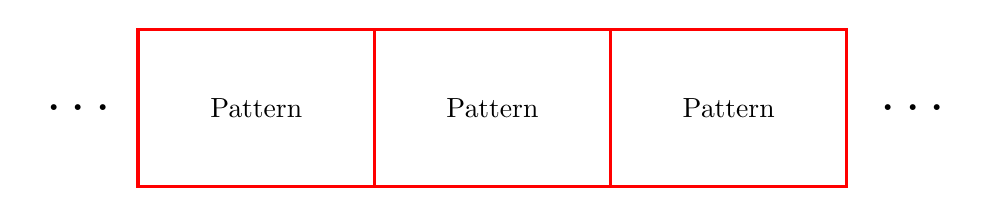
\begin{tikzpicture}
    \node[scale=2] at (-0.2, 1) {\ldots};
    \foreach \j in {0,...,2} {
        \draw[red, very thick] (0.5+3*\j,0) rectangle (3.5+3*\j,2);
        \node at (2 + 3*\j, 1) {Pattern};
    }
    % Add ellipsis at the end
    \node[scale=2] at (10.4, 1) {\ldots};
\end{tikzpicture}

\end{document}
        \caption{Freize groups}
        \label{fig:Freize}
    \end{figure}
\end{frame}

\begin{frame}{Bravais Lattices}
    \begin{figure}
        \centering
        % \resizebox{0.9\columnwidth}{!}{%
        \documentclass[class=beamer, crop=false]{standalone}

\usepackage{tikz}
\usepackage{subcaption}
\usetikzlibrary{calc}


\begin{document}

% \begin{figure}[0.8\linewidth]
  % \centering
  \begin{columns}[t]
      \centering
      \column{0.4\textwidth}
      \centering
    
      \resizebox{0.5\columnwidth}{!}{%
      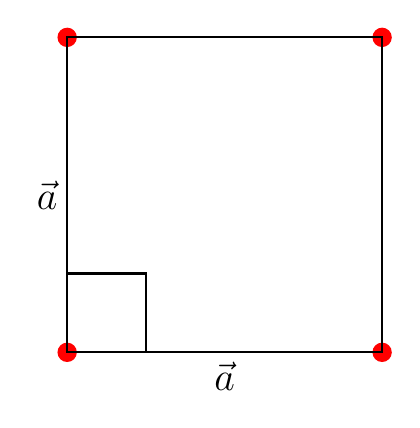
\begin{tikzpicture}
        \def\a{4}  % length of side a
            
        % Calculate the coordinates of the points
        \coordinate (A) at (0, 0);
        \coordinate (B) at (\a, 0);
        \coordinate (C) at (\a, \a);
        \coordinate (D) at (0, \a);
    
        \fill[red]  (A) circle(3.5pt) (B) circle(3.5pt) (C) circle(3.5pt) (D) circle(3.5pt);
            
        % Draw the square unit cell
        \draw[thick] (A) -- (B) -- (C) -- (D) -- cycle;
    
        % Draw right angle
        \draw[thick] (0,1) -- (1,1) -- (1,0);
    
        %Draw lattice parameters
        \node[left] at ($(A)!0.5!(D)$) {\Large $\vec{a}$};
        \node[below] at ($(A)!0.5!(B)$) {\Large $\vec{a}$};
        
      \end{tikzpicture}}
    
      
      \vspace{0.5ex}
    
      {\footnotesize\textbf{(a)} Square Cell}
    
      \column{0.4\textwidth}
        
      \resizebox{0.6\columnwidth}{!}{%
      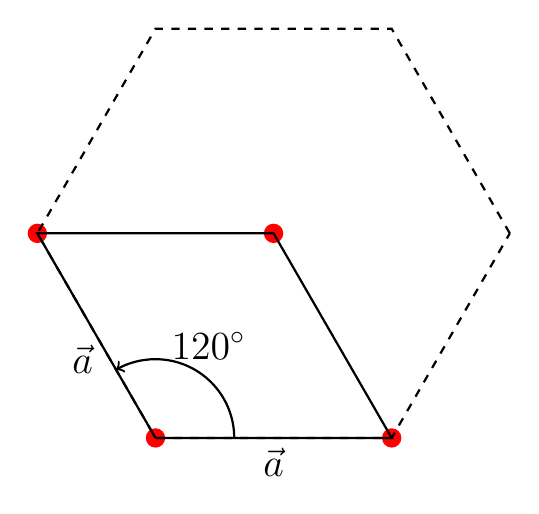
\begin{tikzpicture}
        \def\a{3}  % length of side a
            
        Calculate the coordinates of the points
        \coordinate (A) at (0:\a);
        \coordinate (B) at (60:\a);
        \coordinate (C) at (120:\a);
        \coordinate (D) at (180:\a);
        \coordinate (E) at (240:\a);
        \coordinate (F) at (300:\a);
        \coordinate (G) at (0,0);
       
        % Creates nodes at vertices
        \fill[red]  (D) circle(3.5pt) (E) circle(3.5pt) (F) circle(3.5pt) (G) circle(3.5pt);
        
        % Draw the hexagon boundary
        \draw[thick,dashed] (A) -- (B) -- (C) -- (D) -- (E) -- (F) -- (A);
    
        % Draw the cell
        \draw[thick] (E) -- (F) -- (G) -- (D) -- (E); 
            
        %Draw lattice parameters
        \node[anchor={60}] at ($(D)!0.5!(E)$) {\Large $\vec{a}$};
        \node[below] at ($(E)!0.5!(F)$) {\Large $\vec{a}$};
    
        % Optional: add angle markers
        \draw[thick, ->] (E) ++(1,0) arc[start angle=0, end angle=120, radius=1] node[midway,anchor={-120}] {\Large $120^\circ$};
        
      \end{tikzpicture}}
    
      {\footnotesize\textbf{(b)} Hexagon Cell}
    
    \end{columns}
    \vspace{1em}
    \begin{columns}[t]
      \centering
      \column{0.25\textwidth}
    
      \resizebox{0.9\columnwidth}{!}{%
      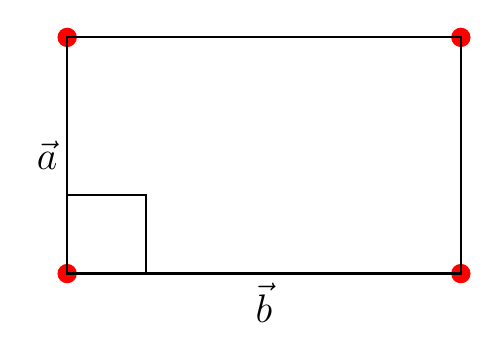
\begin{tikzpicture}
        \def\a{5}  % length of side a
        \def\b{3}  % length of side b
        \def\y{5}
    
        % Calculate the coordinates of the points
        \coordinate (A) at (0, 0);
        \coordinate (B) at (\a, 0);
        \coordinate (C) at (\a, \b);
        \coordinate (D) at (0, \b);
    
        % Creates nodes at vertices
        \fill[red]  (A) circle(3.5pt) (B) circle(3.5pt) (C) circle(3.5pt) (D) circle(3.5pt);
        
        % Draw right angle
        \draw[thick] (0,1) -- (1,1) -- (1,0);
    
        % Draw the rectangular unit cell
        \draw[thick] (A) -- (B) -- (C) -- (D) -- cycle;
       
        %Draw lattice parameters
        \node[left] at ($(A)!0.5!(D)$) {\Large $\vec{a}$};
        \node[below] at ($(A)!0.5!(B)$) {\Large $\vec{b}$};
    
      \end{tikzpicture}}
    
       \vspace{0.5ex}

       % Second row
    
      {\footnotesize\textbf{(c)} Rectangle Cell}
    
      \column{0.25\textwidth}
    
      \resizebox{0.9\columnwidth}{!}{%
      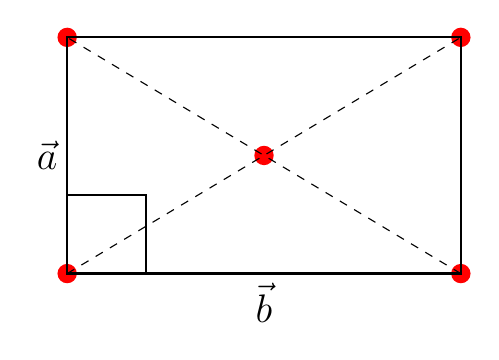
\begin{tikzpicture}
        \def\a{5}  % length of side a
        \def\b{3}  % length of side b
    
        % Calculate the coordinates of the points
        \coordinate (A) at (0, 0);
        \coordinate (B) at (\a, 0);
        \coordinate (C) at (\a, \b);
        \coordinate (D) at (0, \b);
    
        % Creates nodes at vertices
        \fill[red]  (A) circle(3.5pt) (B) circle(3.5pt) (C) circle(3.5pt) (D) circle(3.5pt);
        % Creates nodes at centers
        \fill[red] ($(A)!0.5!(C)$) circle(3.5pt);
    
        % Draw the rectangular unit cell
        \draw[thick] (A) -- (B) -- (C) -- (D) -- cycle;
    
        % Draw lines
        \draw[dashed] (A) -- (C);
        \draw[dashed] (B) -- (D);
    
        % Draw right angle
        \draw[thick] (0,1) -- (1,1) -- (1,0);
            
        %Draw lattice parameters
        \node[left] at ($(A)!0.5!(D)$) {\Large $\vec{a}$};
        \node[below] at ($(A)!0.5!(B)$) {\Large $\vec{b}$};
                
      \end{tikzpicture}}
    
      \vspace{0.5ex}
    
      {\footnotesize\textbf{(d)} Rhombic Cell}
    
      \column{0.3\textwidth}
    
      \resizebox{0.9\columnwidth}{!}{%
      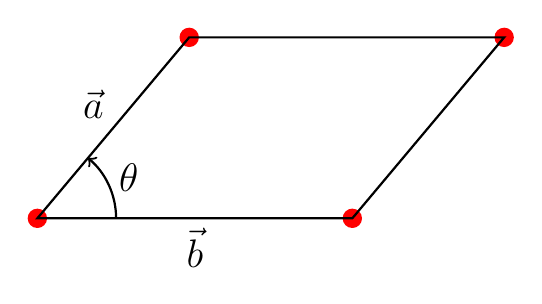
\begin{tikzpicture}
        % Define the lengths of the sides and the angle
        \def\a{4}  % length of side a
        \def\b{3}  % length of side b
        \def\angle{50}  % angle between sides a and b
    
        % Calculate the coordinates of the points
        \coordinate (A) at (0, 0);
        \coordinate (B) at (\a, 0);
        \coordinate (C) at ({\a + \b*cos(\angle)}, {\b * sin(\angle)});
        \coordinate (D) at ({\b * cos(\angle)}, {\b * sin(\angle)});
         
        % Creates nodes at vertices
        \fill[red]  (A) circle(3.5pt) (B) circle(3.5pt) (C) circle(3.5pt) (D) circle(3.5pt);
    
        % Draw the oblique unit cell
        \draw[thick] (A) -- (B) -- (C) -- (D) -- cycle;
    
        %Draw lattice parameters
        \node[anchor={-\angle}] at ($(A)!0.5!(D)$) {\Large $\vec{a}$};
        \node[below] at ($(A)!0.5!(B)$) {\Large $\vec{b}$};
        
        % Optional: add angle markers
        \draw[thick, ->] (A) ++(1,0) arc[start angle=0, end angle=\angle, radius=1] node[midway, anchor={150+\angle}] {\Large $\theta$};
      \end{tikzpicture}}
    
      \vspace{0.5ex}
    
      {\footnotesize\textbf{(e)} Oblique Cell}
    \end{columns}
  % \caption{All five two‐dimensional Bravais unit cells.}
  % \label{fig:bravais-cells}
% \end{figure}

\end{document}

        \caption{All five two‐dimensional Bravais unit cells.}
        \label{fig:bravis-lattices}
    \end{figure}
    % \documentclass[class=beamer, crop=false]{standalone}

\usepackage{tikz}
\usepackage{subcaption}
\usetikzlibrary{calc}


\begin{document}

% \begin{figure}[0.8\linewidth]
  % \centering
  \begin{columns}[t]
      \centering
      \column{0.4\textwidth}
      \centering
    
      \resizebox{0.5\columnwidth}{!}{%
      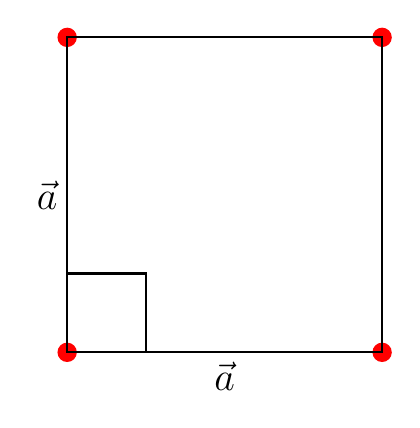
\begin{tikzpicture}
        \def\a{4}  % length of side a
            
        % Calculate the coordinates of the points
        \coordinate (A) at (0, 0);
        \coordinate (B) at (\a, 0);
        \coordinate (C) at (\a, \a);
        \coordinate (D) at (0, \a);
    
        \fill[red]  (A) circle(3.5pt) (B) circle(3.5pt) (C) circle(3.5pt) (D) circle(3.5pt);
            
        % Draw the square unit cell
        \draw[thick] (A) -- (B) -- (C) -- (D) -- cycle;
    
        % Draw right angle
        \draw[thick] (0,1) -- (1,1) -- (1,0);
    
        %Draw lattice parameters
        \node[left] at ($(A)!0.5!(D)$) {\Large $\vec{a}$};
        \node[below] at ($(A)!0.5!(B)$) {\Large $\vec{a}$};
        
      \end{tikzpicture}}
    
      
      \vspace{0.5ex}
    
      {\footnotesize\textbf{(a)} Square Cell}
    
      \column{0.4\textwidth}
        
      \resizebox{0.6\columnwidth}{!}{%
      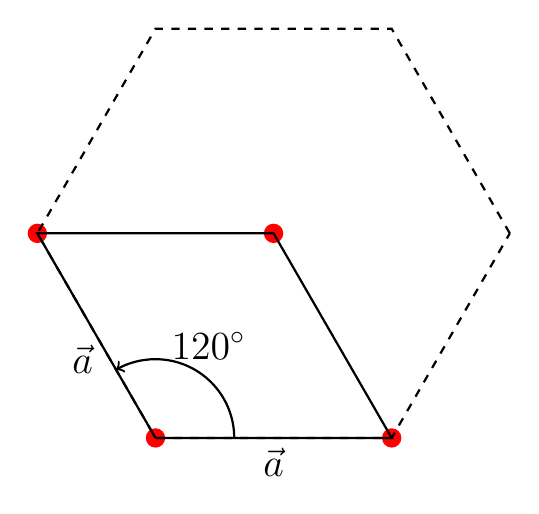
\begin{tikzpicture}
        \def\a{3}  % length of side a
            
        Calculate the coordinates of the points
        \coordinate (A) at (0:\a);
        \coordinate (B) at (60:\a);
        \coordinate (C) at (120:\a);
        \coordinate (D) at (180:\a);
        \coordinate (E) at (240:\a);
        \coordinate (F) at (300:\a);
        \coordinate (G) at (0,0);
       
        % Creates nodes at vertices
        \fill[red]  (D) circle(3.5pt) (E) circle(3.5pt) (F) circle(3.5pt) (G) circle(3.5pt);
        
        % Draw the hexagon boundary
        \draw[thick,dashed] (A) -- (B) -- (C) -- (D) -- (E) -- (F) -- (A);
    
        % Draw the cell
        \draw[thick] (E) -- (F) -- (G) -- (D) -- (E); 
            
        %Draw lattice parameters
        \node[anchor={60}] at ($(D)!0.5!(E)$) {\Large $\vec{a}$};
        \node[below] at ($(E)!0.5!(F)$) {\Large $\vec{a}$};
    
        % Optional: add angle markers
        \draw[thick, ->] (E) ++(1,0) arc[start angle=0, end angle=120, radius=1] node[midway,anchor={-120}] {\Large $120^\circ$};
        
      \end{tikzpicture}}
    
      {\footnotesize\textbf{(b)} Hexagon Cell}
    
    \end{columns}
    \vspace{1em}
    \begin{columns}[t]
      \centering
      \column{0.25\textwidth}
    
      \resizebox{0.9\columnwidth}{!}{%
      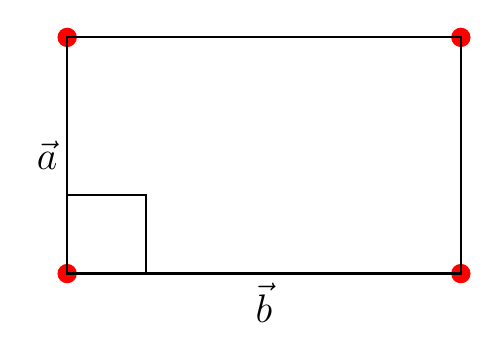
\begin{tikzpicture}
        \def\a{5}  % length of side a
        \def\b{3}  % length of side b
        \def\y{5}
    
        % Calculate the coordinates of the points
        \coordinate (A) at (0, 0);
        \coordinate (B) at (\a, 0);
        \coordinate (C) at (\a, \b);
        \coordinate (D) at (0, \b);
    
        % Creates nodes at vertices
        \fill[red]  (A) circle(3.5pt) (B) circle(3.5pt) (C) circle(3.5pt) (D) circle(3.5pt);
        
        % Draw right angle
        \draw[thick] (0,1) -- (1,1) -- (1,0);
    
        % Draw the rectangular unit cell
        \draw[thick] (A) -- (B) -- (C) -- (D) -- cycle;
       
        %Draw lattice parameters
        \node[left] at ($(A)!0.5!(D)$) {\Large $\vec{a}$};
        \node[below] at ($(A)!0.5!(B)$) {\Large $\vec{b}$};
    
      \end{tikzpicture}}
    
       \vspace{0.5ex}

       % Second row
    
      {\footnotesize\textbf{(c)} Rectangle Cell}
    
      \column{0.25\textwidth}
    
      \resizebox{0.9\columnwidth}{!}{%
      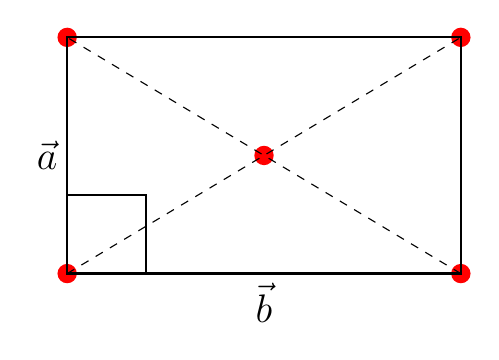
\begin{tikzpicture}
        \def\a{5}  % length of side a
        \def\b{3}  % length of side b
    
        % Calculate the coordinates of the points
        \coordinate (A) at (0, 0);
        \coordinate (B) at (\a, 0);
        \coordinate (C) at (\a, \b);
        \coordinate (D) at (0, \b);
    
        % Creates nodes at vertices
        \fill[red]  (A) circle(3.5pt) (B) circle(3.5pt) (C) circle(3.5pt) (D) circle(3.5pt);
        % Creates nodes at centers
        \fill[red] ($(A)!0.5!(C)$) circle(3.5pt);
    
        % Draw the rectangular unit cell
        \draw[thick] (A) -- (B) -- (C) -- (D) -- cycle;
    
        % Draw lines
        \draw[dashed] (A) -- (C);
        \draw[dashed] (B) -- (D);
    
        % Draw right angle
        \draw[thick] (0,1) -- (1,1) -- (1,0);
            
        %Draw lattice parameters
        \node[left] at ($(A)!0.5!(D)$) {\Large $\vec{a}$};
        \node[below] at ($(A)!0.5!(B)$) {\Large $\vec{b}$};
                
      \end{tikzpicture}}
    
      \vspace{0.5ex}
    
      {\footnotesize\textbf{(d)} Rhombic Cell}
    
      \column{0.3\textwidth}
    
      \resizebox{0.9\columnwidth}{!}{%
      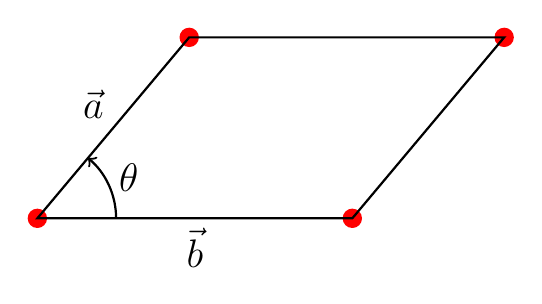
\begin{tikzpicture}
        % Define the lengths of the sides and the angle
        \def\a{4}  % length of side a
        \def\b{3}  % length of side b
        \def\angle{50}  % angle between sides a and b
    
        % Calculate the coordinates of the points
        \coordinate (A) at (0, 0);
        \coordinate (B) at (\a, 0);
        \coordinate (C) at ({\a + \b*cos(\angle)}, {\b * sin(\angle)});
        \coordinate (D) at ({\b * cos(\angle)}, {\b * sin(\angle)});
         
        % Creates nodes at vertices
        \fill[red]  (A) circle(3.5pt) (B) circle(3.5pt) (C) circle(3.5pt) (D) circle(3.5pt);
    
        % Draw the oblique unit cell
        \draw[thick] (A) -- (B) -- (C) -- (D) -- cycle;
    
        %Draw lattice parameters
        \node[anchor={-\angle}] at ($(A)!0.5!(D)$) {\Large $\vec{a}$};
        \node[below] at ($(A)!0.5!(B)$) {\Large $\vec{b}$};
        
        % Optional: add angle markers
        \draw[thick, ->] (A) ++(1,0) arc[start angle=0, end angle=\angle, radius=1] node[midway, anchor={150+\angle}] {\Large $\theta$};
      \end{tikzpicture}}
    
      \vspace{0.5ex}
    
      {\footnotesize\textbf{(e)} Oblique Cell}
    \end{columns}
  % \caption{All five two‐dimensional Bravais unit cells.}
  % \label{fig:bravais-cells}
% \end{figure}

\end{document}

\end{frame}




\begin{frame}{Wallpaper groups}
    \begin{figure}
        \centering
        % \input{diagrams/Wallpaper Group Diagrams/AllGroups}
        \documentclass[class=beamer, crop=false]{standalone}
%\documentclass[12pt]{article}
\usepackage{tikz}
\usepackage{subcaption}
\usetikzlibrary{calc}
\usetikzlibrary {shapes.geometric}
\usepackage{graphicx}
\usepackage{standalone} 


\begin{document}

% \begin{frame}{The 17 Wallpaper Groups}

  % ─── First row: 6 diagrams ───────────────────────────────────────────
  %── p1 ─────────────────────────────────────────────────────────────
  \begin{minipage}[t]{0.20\textwidth}
    \centering
    \includestandalone[width=\linewidth]{diagrams/wallpaper-groups/p1}\\[-0.5ex]
    {\footnotesize\textbf{p1}}
  \end{minipage}%
  \hspace{-0.4em}% ← adjust this
  %── p2 ─────────────────────────────────────────────────────────────
  \begin{minipage}[t]{0.17\textwidth}
    \centering
    \includestandalone[width=\linewidth]{diagrams/wallpaper-groups/p2}\\[-0.5ex]
    {\footnotesize\textbf{p2}}
  \end{minipage}%
  \hspace{0.2em}% ← adjust this
  %── pm ─────────────────────────────────────────────────────────────
  \begin{minipage}[t]{0.15\textwidth}
    \centering
    \includestandalone[width=\linewidth]{diagrams/wallpaper-groups/pm}\\[-0.5ex]
    {\footnotesize\textbf{pm}}
  \end{minipage}%
  \hspace{0.5em}% ← adjust this
  %── pg ─────────────────────────────────────────────────────────────
  \begin{minipage}[t]{0.14\textwidth}
    \centering
    \includestandalone[width=\linewidth]{diagrams/wallpaper-groups/pg}\\[-0.5ex]
    {\footnotesize\textbf{pg}}
  \end{minipage}%
  \hspace{0.2em}% ← adjust this
  %── cm ─────────────────────────────────────────────────────────────
  \begin{minipage}[t]{0.145\textwidth}
    \centering
    \includestandalone[width=\linewidth]{diagrams/wallpaper-groups/cm}\\[-0.5ex]
    {\footnotesize\textbf{cm}}
  \end{minipage}%
  \hspace{0.2em}% ← adjust this
  %── pmm ────────────────────────────────────────────────────────────
  \begin{minipage}[t]{0.15\textwidth}
    \centering
    \includestandalone[width=\linewidth]{diagrams/wallpaper-groups/pmm}\\[-0.5ex]
    {\footnotesize\textbf{pmm}}
  \end{minipage}

  \vspace{1em}

  % ─── Second row: 6 diagrams ──────────────────────────────────────────
  \begin{columns}[t,onlytextwidth]
    \column{0.15\textwidth}\centering
      \includestandalone[width=0.9\columnwidth]{diagrams/wallpaper-groups/pmg}
      \\[-0.5ex]\footnotesize\textbf{pmg}

    \column{0.15\textwidth}\centering
      \includestandalone[width=0.9\columnwidth]{diagrams/wallpaper-groups/pgg}
      \\[-0.5ex]\footnotesize\textbf{pgg}

    \column{0.16\textwidth}\centering
      \includestandalone[width=0.9\columnwidth]{diagrams/wallpaper-groups/cmm}
      \\[-0.5ex]\footnotesize\textbf{cmm}

      \column{0.16\textwidth}\centering
      \includestandalone[width=0.9\columnwidth]{diagrams/wallpaper-groups/p4}
      \\[-0.5ex]\footnotesize\textbf{p4}

    \column{0.16\textwidth}\centering
      \includestandalone[width=0.9\columnwidth]{diagrams/wallpaper-groups/p4m}
      \\[-0.5ex]\footnotesize\textbf{p4m}

    \column{0.16\textwidth}\centering
      \includestandalone[width=0.9\columnwidth]{diagrams/wallpaper-groups/p4g}
      \\[-0.5ex]\footnotesize\textbf{p4g}

  \end{columns}

  \vspace{1em}

  % ─── Third row: 5 diagrams ───────────────────────────────────────────
  \begin{minipage}[t]{0.2\textwidth}
    \centering
    \includestandalone[width=\linewidth]{diagrams/wallpaper-groups/p3}\\[-0.5ex]
    {\footnotesize\textbf{p3}}
  \end{minipage}%
  % \hspace{-0.2em}% <<–– try -0.8em, -1em, -1.2em etc.
  \begin{minipage}[t]{0.19\textwidth}
    \centering
    \includestandalone[width=\linewidth]{diagrams/wallpaper-groups/p3m1}\\[-0.5ex]
    {\footnotesize\textbf{p3m1}}
  \end{minipage}%
  % \hspace{-0.2em}%
  \begin{minipage}[t]{0.2\textwidth}
    \centering
    \includestandalone[width=\linewidth]{diagrams/wallpaper-groups/p31m}\\[-0.5ex]
    {\footnotesize\textbf{p31m}}
  \end{minipage}%
  % \hspace{-0.2em}%
  \begin{minipage}[t]{0.2\textwidth}
    \centering
    \includestandalone[width=\linewidth]{diagrams/wallpaper-groups/p6}\\[-0.5ex]
    {\footnotesize\textbf{p6}}
  \end{minipage}%
  % \hspace{-0.2em}%
  \begin{minipage}[t]{0.2\textwidth}
    \centering
    \includestandalone[width=\linewidth]{diagrams/wallpaper-groups/p6m}\\[-0.5ex]
    {\footnotesize\textbf{p6m}}
  \end{minipage}

% \end{frame}

\end{document}

        \caption{The 17 wallpaper groups }
        \label{fig:17WallpaperGroups}
    \end{figure}
\end{frame}


\begin{frame}{Hilbert problems}
    
\end{frame}

\begin{frame}{Penrose Tilling}
    \begin{figure}
        \centering
        \includegraphics[width=0.5\linewidth]{Pictures/Penrose_Tiling_(Rhombi).svg}
        \caption{Penrose tilling}
        \label{fig:penrose-rhombi}
    \end{figure}
\end{frame}

\begin{frame}{Additionally Resources}
    
\end{frame}

\begin{frame}{References}
    
\end{frame}


\end{document}